\clearpage
\subsection{Prisma: determinazione della lunghezza d'onda per diverse lampade}
\label{sec:prisma2}
Il fascio collimato di lunghezza d'onda incognita viene rifratto attraverso un prisma e viene misurato l'angolo di minima deviazione per calcolare le lunghezze d'onda dello spettro di emissione del gas. Valgono le stesse considerazioni sulle modalità di misura fatte nel paragrafo \ref{sec:prisma1}. Le lampade utilizzate sono la C e la D.\\
\\
Misurato $\delta$, si ottiene la lunghezza d'onda eguagliando le due espressioni dell'indice di rifrazione, con $\alpha$ noto ($62 \pm 1 °$) ed A e B ricavati da esperimento precedente. (Dove è stato sottinteso $\delta = \delta(\lambda)$ per alleggerire la notazione)
    $$ n(\lambda) = \frac{\sin(\frac{\alpha + \delta }{2})}{\sin(\alpha/2) } = A + B/\lambda^2 $$
quindi:
    $$ \frac{1}{\lambda^2} = \frac{\frac{ \sin( (\alpha + \delta)/2 ) }{\sin(\alpha/2) } - A}{B} $$
e:
    $$\lambda = \sqrt{ \frac{B}{ \frac{ \sin( (\alpha + \delta)/2 ) }{\sin(\alpha/2) } -A } } $$
\subsubsection{Lampada C}
Dati:
\begin{table}[H]
\begin{center}
\caption{Dati lampada C}
\begin{tabular}{|c|c|}
\hline
Colore	&	$\delta$	    \\
    	&	rad	            \\
    	&	$\pm 0.003 $	\\ \hline
Rosso1	&	0.830		    \\
Rosso2	&	0.830   	   	\\
Giallo	&	0.841   		\\
Verde1	&	0.847	    	\\
Verde2	&	0.853	    	\\
Verde3	&	0.860    		\\
Verde4	&	0.861		    \\
Blu1	&	0.867	    	\\
Blu2	&	0.876   		\\
Viola	&	0.879	    	\\ \hline
\end{tabular}
\end{center}
\label{label}
\end{table}

Risultati:
\begin{table}[H]
\begin{center}
\caption{Spettro Lampada C}
\begin{tabular}{|c|c|c|}
\hline
Colore & Lungh.Onda [nm] & Errore [nm]\\ 
\hline
Rosso & 680 & 60 \\ 
Giallo & 590 & 40 \\ 
Verde1 & 560 & 30 \\ 
Verde2 & 530 & 20 \\ 
Verde3 & 500 & 20 \\ 
Verde4 & 500 & 20 \\ 
Blu1 & 480 & 20 \\ 
Blu2 & 450 & 10 \\ 
Viola & 440 & 10 \\ 
\hline
\end{tabular}
\end{center}
\label{label}
\end{table}



\subsubsection{Lampada D}
Dati:
\begin{table}[H]
\begin{center}
\caption{Dati lampada D}
\begin{tabular}{|c|c|c|}
\hline
Colore  	&	$\delta$    	\\
	        &	rad		        \\
	        &	$\pm 0.003 $	\\ \hline
Rosso   	&	0.830		    \\
Arancione	&	0.840	    	\\
Giallo  	&	0.841   		\\
Verde1	    &	0.847		    \\
Verde2  	&	0.850	        \\
Blu	        &	0.876   		\\
Viola	    &	0.888	    	\\ \hline
\end{tabular}
\end{center}
\label{label}
\end{table}

Risultati:
\begin{table}[H]
\begin{center}
\caption{Spettro Lampada D}
\begin{tabular}{|c|c|c|}
\hline
Colore & Lungh.Onda [nm] & Errore [nm] \\ 
\hline
Rosso & 680 & 60 \\ 
Arancione & 600 & 40 \\ 
Giallo & 590 & 40 \\ 
Verde1 & 560 & 30 \\ 
Verde2 & 540 & 30 \\ 
Blu & 450 & 10 \\ 
Viola & 420 & 10 \\ 
\hline
\end{tabular}
\end{center}
\label{label}
\end{table}



\subsubsection{Confronto con spettro del visibile}
\label{sec:prisma_confronto}
%
% Spettro lampade C e D
%
    \begin{figure}[H]
    \centering
    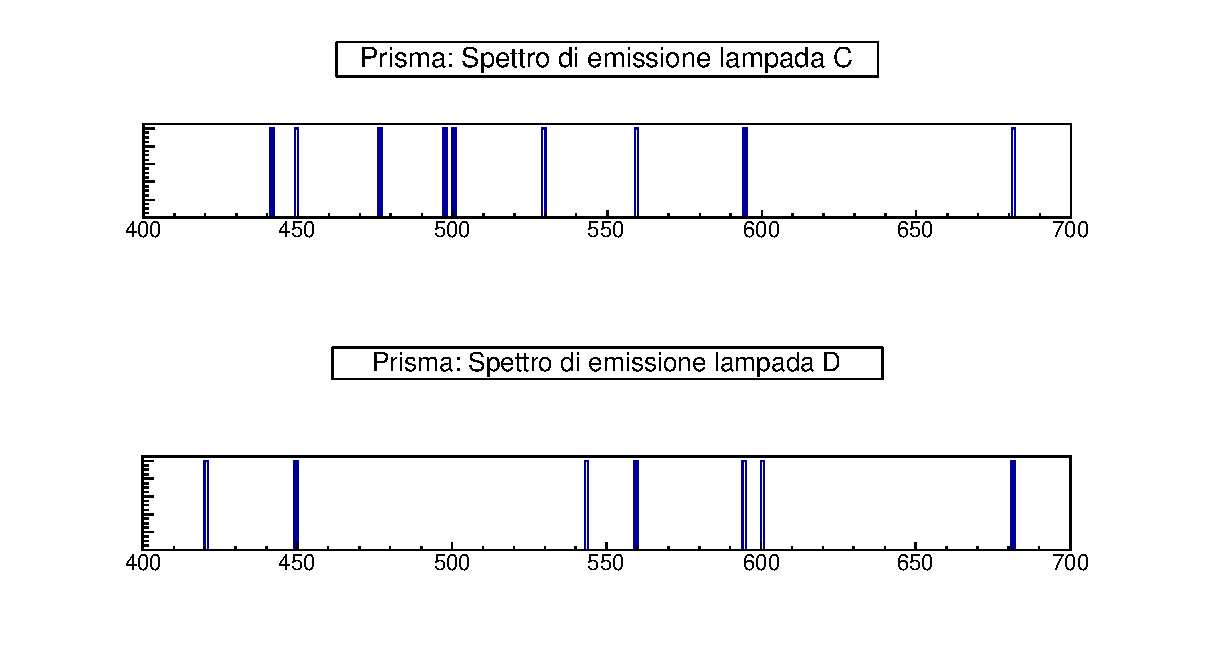
\includegraphics[scale=0.8]{Grafici/O3_P2_2_spectrum.eps}
    %\caption{}
    \includegraphics[scale=1.2]{Grafici/VISspectrum.jpg}
    %\caption{}
    \label{fig:C3_P2_RL}
    \end{figure} 
%
\paragraph{Considerazioni:}{Utilizzando il prisma si possono osservare molte più righe spettrali che con il reticolo, ma di minore intensità. In alcune zone dello spettro (in particolare nel rosso) le linee risultano talmente fitte da sembrare un continuo, rendendo difficile l'individuazione dei singoli massimi. Si è attribuito perciò un errore maggiore a tali zone, stimato dall'ampiezza della banda di colore continuo osservata.}
